\subsubsection{x86}

\myparagraph{MSVC}

Questo e' cio' che si ottiene dopo la compilazione con MSVC 2010:

\lstinputlisting{patterns/04_scanf/1_simple/ex1_MSVC_EN.asm}

\TT{x} e' una variabile locale.

In base allo standard \CCpp deve essere visibile soltanto in questa funzione e non in altri ambiti (esterni alla funzione).
Tradizionalmente, le variabili locali sono memorizzate sullo stack. 
Ci sono probabilmente altri modi per allocarle, ma in x86 e' cosi'.

\myindex{x86!\Instructions!PUSH}
Lo scopo dell'istruzione che segue il prologo della funzione, \TT{PUSH ECX}, non e' quello di salvare lo stato di \ECX  
(si noti infatti l'assenza della corrispondente istruzione \TT{POP ECX} alla fine della funzione).

Infatti alloca 4 byte sullo stack per memorizzare la variabile \TT{x}.

\label{stack_frame}
\myindex{\Stack!Stack frame}
\myindex{x86!\Registers!EBP}
\TT{x} sara' acceduta con l'aiuto della macro \TT{\_x\$} (che e' uguale a -4) ed il registro \EBP che punta al frame corrente.

Durante l'esecuzione delle funziona, \EBP punta allo \gls{stack frame} corrente 
rendendo possibile accedere alle variabili locali ed agli argomenti della funzione attraverso \TT{EBP+offset}.

\myindex{x86!\Registers!ESP}
E' anche possibile usare \ESP per lo stesso scopo, tuttavia non e' molto conveniente poiche' cambia di frequente.
Il valore di \EBP puo' essere pensato come uno \IT{stato congelato} del valore in \ESP all'inizio dell'esecuzione della funzione.

% FIXME1 это уже было в 02_stack?
Questo e' un tipico layout di uno \gls{stack frame} in un ambiente a 32-bit:

\begin{center}
\begin{tabular}{ | l | l | }
\hline
\dots & \dots \\
\hline
EBP-8 & local variable \#2, \MarkedInIDAAs{} \TT{var\_8} \\
\hline
EBP-4 & local variable \#1, \MarkedInIDAAs{} \TT{var\_4} \\
\hline
EBP & saved value of \EBP \\
\hline
EBP+4 & return address \\
\hline
EBP+8 & \argument \#1, \MarkedInIDAAs{} \TT{arg\_0} \\
\hline
EBP+0xC & \argument \#2, \MarkedInIDAAs{} \TT{arg\_4} \\
\hline
EBP+0x10 & \argument \#3, \MarkedInIDAAs{} \TT{arg\_8} \\
\hline
\dots & \dots \\
\hline
\end{tabular}
\end{center}

La funzione \scanf nel nostro esempio ha due argomenti.
Il primo e' un puntatore alla stringa contenente \TT{\%d} e il secondo e' l'indirizzo della variabile \TT{x}.

\myindex{x86!\Instructions!LEA}
Per prima cosa l'indirizzo della variabile \TT{x} e' caricato nel registro \EAX dall'istruzione \TT{lea eax, DWORD PTR \_x\$[ebp]}.

\LEA sta per \IT{load effective address}, ed e' spesso usata per formare un indirizzo ~(\myref{sec:LEA}).

Potremmo dire che in questo caso \LEA memorizza semplicemente la somma del valore nel registro \EBP e della macro \TT{\_x\$} nel registro \EAX.

E' l'equivalente di \INS{lea eax, [ebp-4]}.

Quindi, 4 viene sottratto dal valore del registro \EBP ed il risultato e' memorizzato nel registro \EAX.
Successivamente il registro \EAX e' messo sullo stack (push) e \scanf viene chiamata.

\printf viene chiamata subito dopo con il suo primo argomento --- un puntatore alla stringa:
\TT{You entered \%d...\textbackslash{}n}.

Il secondo argomento e' preparato con: \TT{mov ecx, [ebp-4]}.
L'istruzione memorizza il valore della variabile \TT{x},  non il suo indirizzo, nel registro \ECX.

Successivamente il valore in \ECX e' memorizzato sullo stack e l'ultima \printf viene chiamata.

\clearpage
\subsection{MSVC + \olly}
\index{\olly}

\RU{Попробуем этот же пример в}\EN{Let's try this example in} \olly.
\RU{Загружаем, нажимаем F8 (\stepover) до тех пор, пока не окажемся в своем исполняемом файле,
а не в}\EN{Let's load it and keep pressing F8 (\stepover) until we reach our executable file
instead of} \TT{ntdll.dll}.
\RU{Прокручиваем вверх до тех пор, пока не найдем \main}\EN{Scroll up until \main appears}.
\RU{Щелкаем на первой инструкции (\TT{PUSH EBP}), нажимаем F2 (\IT{set a breakpoint}), 
затем F9 (\IT{Run}) и точка останова срабатывает на начале \main.}
\EN{Click on the first instruction (\TT{PUSH EBP}), press F2 (\IT{set a breakpoint}), 
then F9 (\IT{Run}).
The breakpoint will be triggered when \main begins.}

\RU{Трассируем до того места, где готовится адрес переменной $x$}%
\EN{Let's trace to the point where the address of the variable $x$ is calculated}:

\begin{figure}[H]
\centering
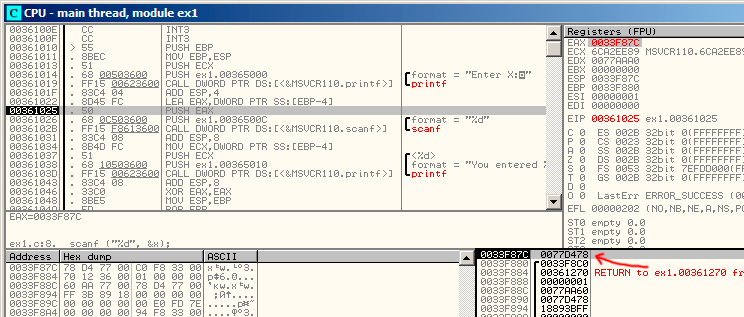
\includegraphics[scale=\FigScale]{patterns/04_scanf/1_simple/ex1_olly_1.png}
\caption{\olly: \RU{вычисляется адрес локальной переменной}\EN{The address of the local variable is calculated}}
\label{fig:scanf_ex1_olly_1}
\end{figure}

\RU{На \EAX в окне регистров можно нажать правой кнопкой и далее выбрать}
\EN{Right-click the \EAX in the registers window and then select} \q{Follow in stack}.
\RU{Этот адрес покажется в окне стека.}
\EN{This address will appear in the stack window.}
\RU{Смотрите, это переменная в локальном стеке. Я нарисовал там красную стрелку}\EN{The red arrow, I have added, points to the variable in the local stack}.
\RU{И там сейчас какой-то мусор}\EN{At that moment this location contains some garbage} (\TT{0x6E494714}).
\RU{Адрес этого элемента стека сейчас, при помощи \PUSH запишется в этот же стек рядом}%
\EN{Now with the help of \PUSH instruction the address of this stack element is going to be stored to the same stack on the next position}.
\RU{Трассируем при помощи F8 вплоть до конца исполнения \scanf}\EN{Let's trace with F8 until the \scanf execution completes}.
\RU{А пока \scanf исполняется, в консольном окне, вводим, например, 123}%
\EN{During the \scanf execution, we input, for example, 123, in the console window}:

\begin{figure}[H]
\centering
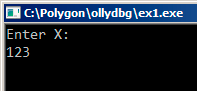
\includegraphics[scale=\NormalScale]{patterns/04_scanf/1_simple/ex1_olly_2.png}
\caption{\RU{Ввод пользователя в консольном окне}\EN{User input in the console window}}
\label{fig:scanf_ex1_olly_2}
\end{figure}

\clearpage
\RU{Вот тут }\scanf \RU{отработал}\EN{completed its execution already}:

\begin{figure}[H]
\centering
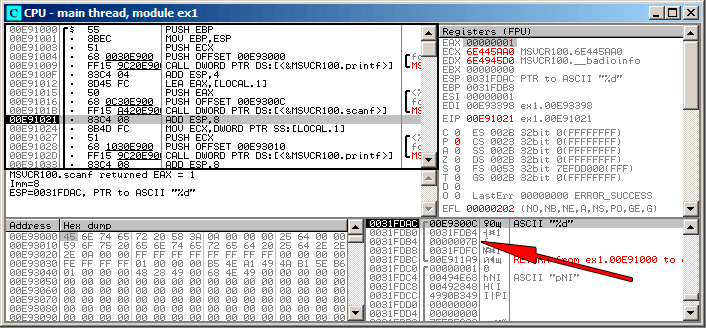
\includegraphics[scale=\FigScale]{patterns/04_scanf/1_simple/ex1_olly_3.png}
\caption{\olly: \scanf \RU{исполнилась}\EN{executed}}
\label{fig:scanf_ex1_olly_3}
\end{figure}

\scanf \RU{вернул}\EN{returns} $1$ \InENRU \EAX, \RU{что означает, что он успешно прочитал одно 
значение}\EN{which implies that it has read successfully one value}.
\RU{В наблюдаемом нами элементе стека теперь}\EN{If we look again at the stack element corresponding to the local variable it now contains} \TT{0x7B} (123).

\clearpage
\RU{Чуть позже это значение копируется из стека в регистр \ECX и передается в \printf}
\EN{Later this value is copied from the stack to the \ECX register and passed to \printf}:

\begin{figure}[H]
\centering
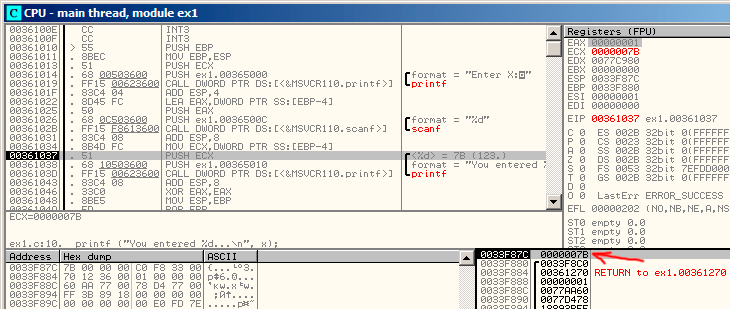
\includegraphics[scale=\FigScale]{patterns/04_scanf/1_simple/ex1_olly_4.png}
\caption{\olly: \RU{готовим значение для передачи в}\EN{preparing the value for passing to} \printf}
\label{fig:scanf_ex1_olly_4}
\end{figure}


\myparagraph{GCC}

Proviamo a compilare questo codice con GCC 4.4.1 su Linux:

\lstinputlisting{patterns/04_scanf/1_simple/ex1_GCC.asm}

\myindex{puts() instead of printf()}
GCC ha sostituito la chiamata a \printf con \puts. La ragione per cui cio' avviene e' stata spiegata in ~(\myref{puts}).

% TODO: rewrite
%\RU{Почему \scanf переименовали в \TT{\_\_\_isoc99\_scanf}, я честно говоря, пока не знаю.}
%\EN{Why \scanf is renamed to \TT{\_\_\_isoc99\_scanf}, I do not know yet.}
% 
% Apparently it has to do with the ISO c99 standard compliance. By default GCC allows specifying a standard to adhere to.
% For example if you compile with -std=c89 the outputted assmebly file will contain scanf and not __isoc99__scanf. I guess current GCC version adhares to c99 by default.
% According to my understanding the two implementations differ in the set of suported modifyers (See printf man page)

Come nell'esempio compilato con MSVC ---gli argomenti sono messi sullo stack utilizzando l'istruzione \MOV.


